\documentclass[12pt]{article}

\usepackage[english]{babel}
\usepackage[utf8x]{inputenc}
\usepackage{amsmath}
\usepackage{graphicx}
\usepackage[margin=1.0in]{geometry}
\usepackage{authblk}

\usepackage{fancyvrb}
\usepackage{color}
<< pygments['pastie.tex'] >>

\title{The IPython Notebook: open, reproducible scientific computing}
\author[1]{Matthias Bussonnier}
\author[2]{Jonathan Frederic}
\author[3]{Bradley M. Froehle}
\author[2]{Brian E. Granger}
\author[3]{Paul Ivanov}
\author[3]{Thomas Kluyver}
\author[3]{Fernando Perez}
\author[3]{Benjamin Ragan-Kelley}
\author[2]{Zachary Sailer}
\affil[1]{Affiliation of Matthias}
\affil[2]{Cal Poly State University}
\affil[3]{University of CA, Berkeley}

\renewcommand\Authands{ and }

\begin{document}
\maketitle

\begin{abstract}
While computing has become a foundation of all it is challenging for researchers . 
\end{abstract}

\section{Introduction}

Scientific research has become pervasively computational. In addition
to experiment and theory, the notions of simulation and data-intensive
discovery have emerged as third and fourth pillars of science \cite{4th-paradigm}.
Today, even theory and experiment are computational, as virtually
all experimental work requires computing (whether in data collection,
pre-processing or analysis) and most theoretical work requires symbolic
and numerical support to develop and refine models. Scanning the pages
of any major scientific journal, one is hard-pressed to find a publication
in any discipline that doesn't depend on computing for its findings.

And yet, for all its importance, computing is often treated as an 
afterthought both in the training of our scientists and in the conduct
of everyday research. Most working scientists have witnessed how computing
is seen as a task of secondary importance that students and postdocs
learn ``on the go'' with little training to ensure that results
are trustworthy, comprehensible and ultimately a solid foundation
for reproducible outcomes. Software and data are stored with poor
organization, documentation and tests. A patchwork of software tools
is used with limited attention paid to capturing the complex workflows
that emerge, and the evolution of code is often not tracked over time,
making it difficult to understand how a result was obtained. Finally,
many of the software packages used by scientists in research are proprietary
and closed-source, preventing the community from having a complete
understanding of the final scientific results. The consequences of
this cavalier approach are serious. Consider, just to name two widely
publicized cases, the loss of public confidence in the ``Climategate''
fiasco \cite{Hef10} or the Duke cancer trials scandal, where sloppy
computational practices likely led to severe health consequences for
several patients \cite{Cou10}. 

This is a large and complex problem that requires changing the educational
process for new scientists, the incentive models for promotions and
rewards, the publication system, and more. We do not aim to tackle
all of these issues here, but our belief is that a central element
of this problem is the nature and quality of the software tools available
for computational work in science. 

\section{Computing and the lifecycle of research}

Based on our experience over the
last decade as practicing researchers, educators and software developers,
we propose an integrated approach to computing where the entire life-cycle
of scientific research is considered, from the initial exploration
of ideas and data to the presentation of final results. Briefly, this
life-cycle can be broken down into the following phases:
\begin{itemize}
\item \textbf{Individual exploration:} a single investigator tests an idea,
algorithm or question, likely with a small-scale test data set or
simulation.
\item \textbf{Collaboration:} if the initial exploration appears promising,
more often than not some kind of collaborative effort ensues.
\item \textbf{Production-scale execution:} large data sets and complex simulations
often require the use of clusters, supercomputers or cloud resources
in parallel.
\item \textbf{Publication:} whether as a paper or an internal report for
discussion with colleagues, results need to be presented to others
in a coherent form.
\item \textbf{Education:} ultimately, research results become part of the
corpus of a discipline that is shared with students and colleagues,
thus seeding the next cycle of research.
\end{itemize}
In this project, we tackle the following problem.\textbf{ There are
no software tools capable of spanning the entire lifecycle of computational
research.} The result is that researchers are forced to use a large
number of disjoint software tools in each of these phases in an awkward
workflow that hinders collaboration and reduces efficiency, quality,
robustness and reproducibility.

These can be illustrated with an example: a researcher might use Matlab
for prototyping, develop high-performance code in C, run post-processing
by twiddling controls in a Graphical User Interface (GUI), import
data back into Matlab for generating plots, polish the resulting plots
by hand in Adobe Illustrator, and finally paste the plots into a publication
manuscript or PowerPoint presentation. But what if months later the
researcher realizes there is a problem with the results? What are
the chances they will be able to know what buttons they clicked, to
reproduce the workflow that can generate the updated plots, manuscript
and presentation? What are the chances that other researchers or students
could reproduce these steps to learn the new method or understand
how the result was obtained? How can reviewers validate that the programs
and overall workflow are free of errors? Even if the researcher successfully
documents each program and the entire workflow, they have to carry
an immense cognitive burden just to keep track of everything.

\section{The IPython Notebook}

We propose that the open source IPython project \cite{PER-GRA:2007}
offers a solution to these problems; a single software tool capable
of spanning the entire life-cycle of computational research. Amongst
high-level open source programming languages, Python is today the
leading tool for general-purpose source scientific computing (along
with R for statistics), finding wide adoption across research disciplines,
education and industry and being a core infrastructure tool at institutions
such as CERN and the Hubble Space Telescope Science Institute \cite{Perez2011,ganga09,SST}.
The PIs created IPython as a system for interactive and parallel computing
that is the\emph{ de facto} environment for scientific Python. In
the last year we have developed the IPython Notebook, a web-based\emph{
interactive computational notebook} that combines code, text, mathematics,
plots and rich media into a single document format (see Fig.~\ref{fig:IPython-notebook}).
The IPython Notebook was designed to enable researchers to move fluidly
between all the phases of the research life-cycle and has gained rapid
adoption. It provides an integrated environment for all computation,
without locking scientists into a specific tool or format: Notebooks
can always be exported into regular scripts and IPython supports the
execution of code in other languages such as R, Octave, bash, etc.
In this project we will expand its capabilities and relevance in the
following phases of the research cycle: interactive exploration, collaboration,
publication and education.

\subsection{Web application}

%\begin{figure}
%\begin{centering}
%\includegraphics[width=3.2in]{fig/ipython-notebook-specgram}
%\par\end{centering}
%
%\caption{\label{fig:IPython-notebook}The web-based IPython Notebook combines
%explanatory text, mathematics, multimedia, code and the results from
%executing the code.}
%\end{figure}

\subsection{Notebook document format}

\subsection{Display architecture}

\subsection{Installation}

\section{Collaboration}

\section{Broader ecosystem}

\section{Future directions}

\section*{Dexy Snippets}

<% set nb = d["notebooks/Chapter1_Introduction.ipynb|ipynb"].from_json() -%>

This notebook uses format \verb|<< nb.nbformat >>|.

\subsection*{Markdown Content}

Here is an example of a markdown cell:

<< d['notebooks/Chapter1_Introduction--42.md'] >>

Here is the same cell in a Verbatim block:

\begin{Verbatim}
<< d['notebooks/Chapter1_Introduction--42.md'] >>
\end{Verbatim}

Here is the same cell presented as highlighted markup:

<< d['notebooks/Chapter1_Introduction--42.md|pyg|l'] >>

\subsection*{Python Content}

<< d['notebooks/Chapter1_Introduction--7-input.py|pyg|l'] >>

\begin{Verbatim}
<< d['notebooks/Chapter1_Introduction--7-output-0.txt'] >>
\end{Verbatim}

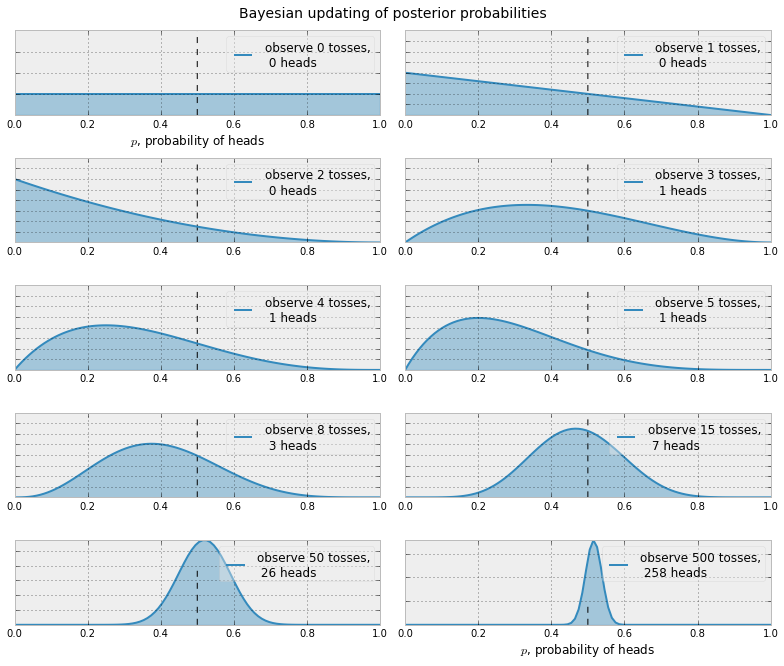
\includegraphics{notebooks/Chapter1_Introduction--7-output-1.png}

\subsection*{Iterating over Cells and Documents}

This notebook has << len(nb.cells) >> cells and << len(nb.documents) >> documents based on these cells.

\subsubsection*{Cells}

Here is a list of cells:

\begin{itemize}
<% for cell in nb.cells -%>
\item{\verb|<< cell >>|}
<% endfor -%>
\end{itemize}

\subsubsection*{Documents}

Here is a list of documents:

\begin{itemize}
<% for doc in nb.documents -%>
\item{\verb|<< doc >>|}
<% endfor -%>
\end{itemize}

Here are the contents of documents:

<% for doc in nb.documents -%>

Here are the contents of \verb|<< doc >>|:

<% if doc.endswith(".py") or doc.endswith(".md") -%>
<< d[doc + "|pyg|l"] >>
<% elif doc.endswith(".png") -%>
\includegraphics{<< doc >>}
<% elif doc.endswith(".txt") -%>
\begin{Verbatim}
<< d[doc] >>
\end{Verbatim}
<% else -%>
Please add a display format for << doc >>.
<% endif -%>
<% endfor -%>

\end{document}
